\documentclass{beamer}
\usepackage{mathrsfs,xcolor,setspace,comment,centernot,listings,framed,subfig,ragged2e}
\usepackage[utf8]{inputenc}
\usepackage[T1]{fontenc}

\DeclareMathOperator{\Cov}{Cov}
\DeclareMathOperator{\Var}{Var}
\DeclareMathOperator{\E}{\mathbb{E}}
\DeclareMathOperator{\Proba}{\mathbb{P}}

\newcommand{\Covb}[2]{\ensuremath{\Cov\!\left[#1,#2\right]}}
\newcommand{\Eb}[1]{\ensuremath{\E\!\left[#1\right]}}
\newcommand{\Pb}[1]{\ensuremath{\Proba\!\left[#1\right]}}
\newcommand{\Varb}[1]{\ensuremath{\Var\!\left[#1\right]}}

% norm
\newcommand{\norm}[1]{\| #1 \|}

\newcommand{\indep}{\rotatebox[origin=c]{90}{$\models$}}



% config du theme metropolis
\usetheme[progressbar=frametitle,block=fill, titleformat=smallcaps,sectionpage=progressbar,]{metropolis}


\title{A generic and modular simulation model for suburban densification}
\subtitle{}

\date{11/03/2025\\
\textit{Journée de la Recherche UGE-IGN-ENSG 2025}\\
Session: Simulating Social and Spatial Processes}

\author{Juste Raimbault\textsuperscript{1,2,3,4}, Vera Götze\textsuperscript{1} and Julien Perret\textsuperscript{1,5}}
\institute{\textsuperscript{1}LaSTIG, IGN-ENSG-UGE\\
\textsuperscript{2}CASA, UCL\\
\textsuperscript{3}UPS CNRS 3611 ISC-PIF\\
\textsuperscript{4}UMR CNRS 8504 Géographie-cités\\
\textsuperscript{5}LaDéHiS, EHESS
}



%definition de la couleur du texte dans la balise \alert{}
\definecolor{vertIGN}{HTML}{96C31E} % vert IGN %vrai valeur #97BE0D
\setbeamercolor{alerted text}{fg=vertIGN}

\definecolor{grisIGN}{HTML}{22292F} % Gris IGN tiré vers le noir 
\setbeamercolor{background canvas}{bg=grisIGN}


% code pour placer le log ENSG dans le bandeau de titre 
\makeatletter
\setbeamertemplate{frametitle}{%
  \nointerlineskip%
  \begin{beamercolorbox}[%
      wd=\paperwidth,%
      sep=0pt,%
      leftskip=\metropolis@frametitle@padding,%
      rightskip=\metropolis@frametitle@padding,%
    ]{frametitle}%
  \metropolis@frametitlestrut@start%
  \insertframetitle%
  \nolinebreak%
  \metropolis@frametitlestrut@end%
  \hfill
  \raisebox{-0.6ex}{
\includegraphics[height=4ex,keepaspectratio]{figures/logoENSG_small.jpg}}
  \end{beamercolorbox}%
}


\newcommand{\noun}[1]{\textsc{#1}}
\newcommand{\jitem}[1]{\item \begin{justify} #1 \end{justify} \vfill{}}
\newcommand{\sframe}[2]{\frame{\frametitle{#1} #2}}

\newenvironment{centercolumns}{\begin{columns}[c]}{\end{columns}}
%\newenvironment{jitem}{\begin{justify}\begin{itemize}}{\end{itemize}\end{justify}}



\usepackage{pifont}
\newcommand{\cmark}{\ding{51}}
\newcommand{\xmark}{\ding{55}}


\usepackage{multirow}

\makeatother




% logo ENSG première page 
\titlegraphic{\vspace{4cm}\flushright
\includegraphics[width=2cm,height=2cm]{figures/logoENSG_big.png}} 





\begin{document}
\metroset{background=dark} % change background theme according to manual
\maketitle	



%  Suburban densification is a process important for urban sustainability, for example to limit urban sprawl and increase public transport ridership. Its dynamics remain difficult to grasp as many stakeholders at different scales are involved, from home and land owners to developpers and public authorities. They furthermore can change drastically with the context and country. We propose in this contribution a formal description of an agent-based simulation model, aimed at capturing such processes with enough genericity to be applied across 3 European countries (France, UK and Germany, studied in the context of the Subdense research project). The modular architecture allows including submodels for specific computations, such as the SimPLU3d model for densification potential and the ParcelManager model for land division. We expect this first proposal to be refined after its application to case studies and its calibration on empirical data, and a discussion with qualitative researchers working with densification stakeholders.

\sframe{Context: the SUBDENSE project}{

\medskip

\begin{columns}
	\begin{column}{0.6\textwidth}
		The SubDense European project studies the dynamics of suburban densification by:
 
	\end{column}
	\begin{column}{0.4\textwidth}
		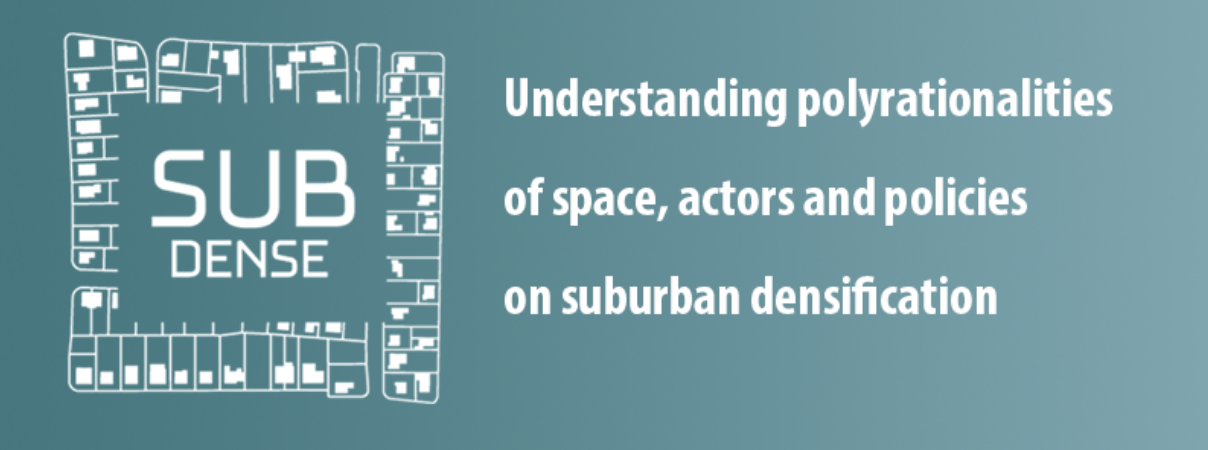
\includegraphics[height=0.2\textheight]{figures/subdense.png}
	\end{column}
\end{columns}


\begin{itemize} 
	\item exploring how diverse strategies of land policy interact with landowners’ and local stakeholders’ interest and agency to shape suburban densification and their impact on suburbia across different planning systems (France, Germany, UK);
	\item combining quantitative approaches (geodata analysis and geosimulation) with qualitative approaches (social and policy science and planning).
\end{itemize}

\bigskip

\centering


\includegraphics[height=0.1\textheight]{figures/logos.png}\hspace{-0.1cm}

\includegraphics[height=0.1\textheight]{figures/tud.png}


}

\sframe{A collaborative dashboard for mediation}{


% Change detection

\begin{columns}
	\begin{column}{0.6\linewidth}
		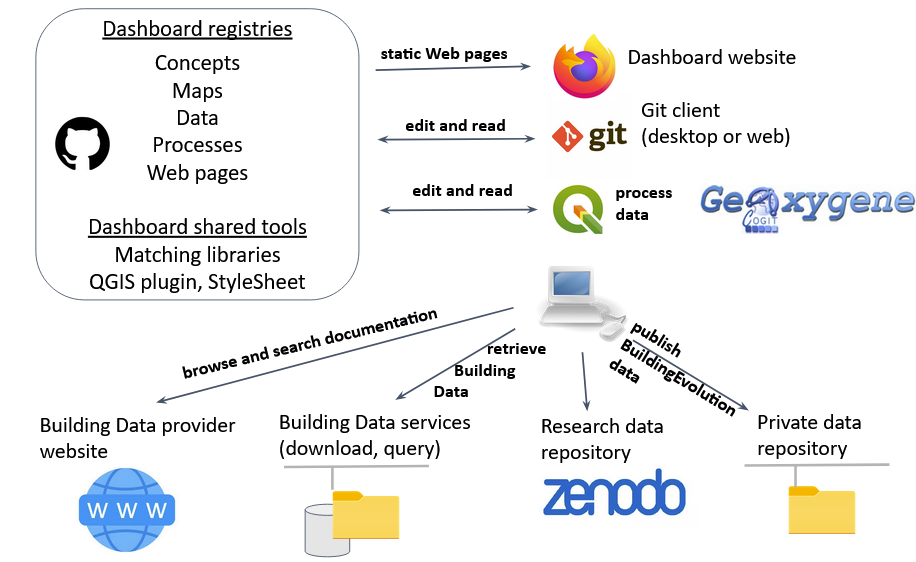
\includegraphics[width=\textwidth]{figures/dashboard.png}\medskip
		
		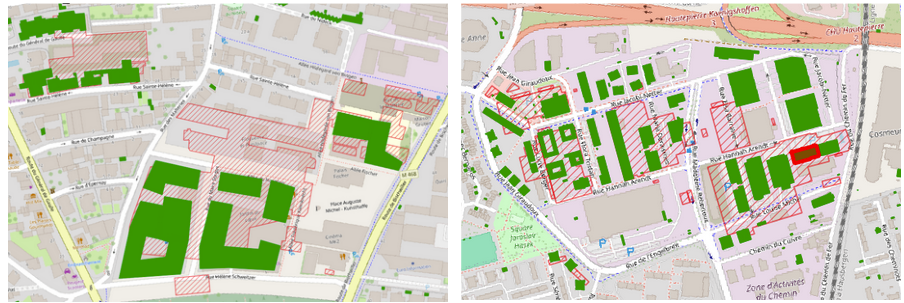
\includegraphics[width=\textwidth]{figures/buildingchange.png}
	\end{column}
	\begin{column}{0.4\linewidth}
	
		\footnotesize	
	
		$\rightarrow$ git-based architecture to share in a reproducible, transparent, and traceable way informations between experts on data products, metadata, code for processing data, etc. \cite{bucher2024conceptualising}
	
		\bigskip
		\bigskip
		
		$\rightarrow$ matching algorithms for building change detection \cite{guardiola2024benchmarking} (cf presentation in session on Change Detection)
	
	\end{column}
\end{columns}

}




\sframe{Research objective}{

% WP3 and obejctive of the ABM

\textbf{WP3 of the Subdense project: } ``\textit{How do land policies respond to the interests and agency of stakeholders in an effective and efficient way?}''

\bigskip

$\rightarrow$ simulation as a tool to explore ``what-if'' scenarios for policies

\medskip

$\rightarrow$ as for qualitative analysis and geospatial data analysis, a generic and transferable approach must be proposed

\bigskip

\textbf{Research question: }

\textit{Which simulation model for densification processes to ensure comparability across countries and the exploration of policies?}


}


\sframe{Simulating urban densification}{

% literature

\begin{itemize}
	\item \cite{burke20243d}: Agent-based Model simulating the behavior of residents, developers, landowners, and the local zoning authority
	\item \cite{leao2018agent}: parcels and buildings as autonomous agents
	\item \cite{curie2010simulation}: simulation at the block level
	\item  \cite{pawar2023analysis}: data driven abm of household relocation and its impact on density
	\item \cite{chakraborty2022cellular}: Cellular Automaton models to model and predict urban densification
	\item \cite{chakraborty2025model}: spatial statistics and machine learning
\end{itemize}





}





\sframe{Model description following the ODD protocol}{

\textit{Overview, Design, Details}: a protocol to describe ABMs in a standardised way \cite{grimm2020odd}
% thght: what matters is interoperable?

\bigskip

\centering

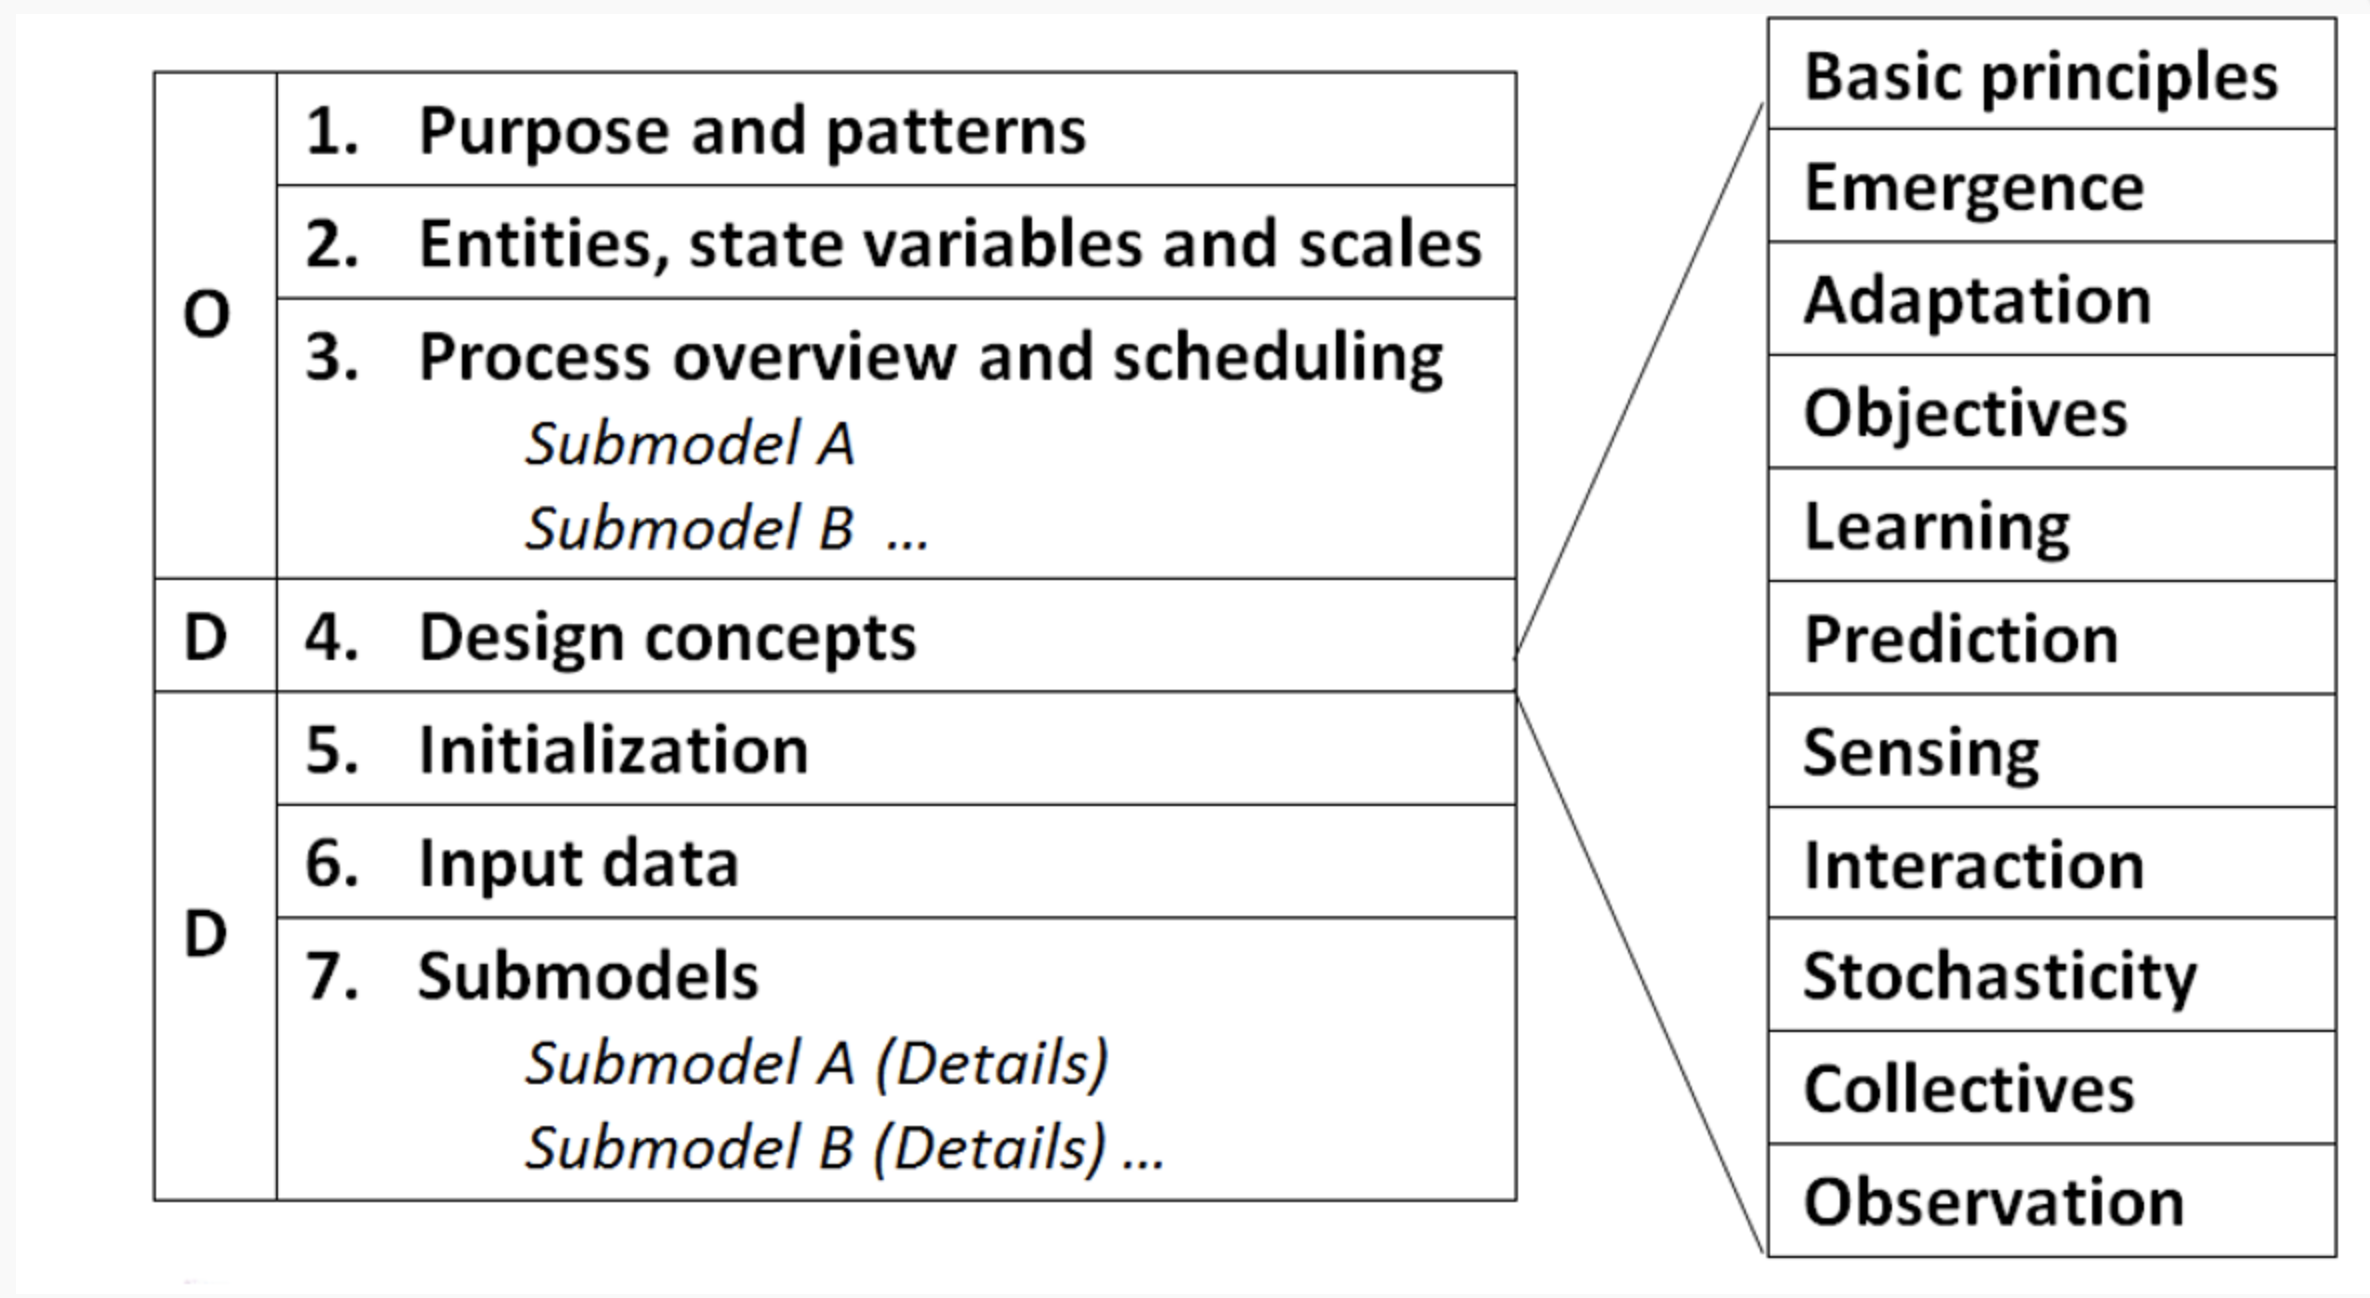
\includegraphics[width=0.9\textwidth]{figures/odd.png}

}

\sframe{Overview}{

\textbf{1. Purpose and patterns: } spatial patterns of densification linked to driver variables and sustainability indicators, to explore and optimise policies linked to densification.

\smallskip

\textbf{2. Entities, state variables and scales: } all agents at the microscopic scale (intra-urban) within an urban area extent (mesoscopic scale) \cite{pumain2008socio}:

\begin{itemize}
	\item City authority (monitoring indicators to adapt regulations: density threshold, financial incentives, ZAN, ZAC, \ldots)
	\item Developers (optimising constructed floor space: develop empty plots or densify/refurbish existing buildings; competition between developers?)
	\item Individual owners (move out, densify their houses, split their plots)
	\item \textbf{Buildings and Plots} are basic geographical entities without autonomous behavior
\end{itemize}



}


\sframe{Overview}{

\textbf{3. Process overview and scheduling: }

\begin{enumerate}
	\item If time step is a multiple of $t_P$, authority updates the regulation (strategy parameters: ``limit sprawl'' (increase density threshold), ``maximise accessibility'' (subsidised development projects), \ldots
	\item Developers with a fixed budget:
	\begin{itemize}
		\item Evaluate a set of areas for potential projects (SimPLU3D model for building potential \cite{brasebin2017apports})
		\item Construct the more profitable development with a price signal $p = floor \times f(density, accessibility, \ldots)$
	\end{itemize}
	\item Landowners (randomly selected) need more space and either move out, densify, or split their plot (ParcelManager model \cite{colomb2022parcel})
\end{enumerate}

}


\sframe{Design concepts}{

\textbf{4. Design concepts:}

\footnotesize

\textbf{Basic principles: } highly simplified ``economic behavior'' of agents, with an accurate spatialisation

\textbf{Emergence: } densification dynamics

\textbf{Adaptation: } locations of agent choices depend on the situation

\textbf{Objectives: } contradictory objectives across agents

\textbf{Learning: } no learning, stationary behavior

\textbf{Prediction: } no prediction, react to the current situation

\textbf{Sensing: } price signal spatially known with noise

\textbf{Interaction: } between agents through the environment (regulations, buildings and plots, prices)

\textbf{Stochasticity: } randomness in choices (type ``discrete choices'')

\textbf{Collectives: } no endogeneous collective, strong emergence postulated with the authority

\textbf{Observation: } spatio-temporal distribution of density and prices

}

\sframe{Details}{

\footnotesize

\textbf{5. Initialisation: } plots and buildings (single-family houses and multi-storeys), one authority, a few developers, landowners a fixed proportion of dwellings

\smallskip

\textbf{6. Input data: }

\begin{itemize}
	\item synthetic data to remove geographical contingencies \cite{raimbault2019space}: from a density landscape \cite{raimbault2018calibration} or directly buildings \cite{raimbault2019generating}
	\item real plots and buildings from an urban area, filled with a synthetic population of landowners \cite{colomb2024projet}
\end{itemize}

\smallskip

\textbf{7. Submodels: }

\begin{itemize}
	\item SimPLU3D to evaluate densification potential \cite{brasebin2017apports}
	\item ParcelManager for splitting plots \cite{colomb2022parcel}
	\item Economic models for prices, developers behavior and utility, landowners discrete choices and utility
	%\item \ldots
\end{itemize}

$\rightarrow$ submodels can be included or not in a multi-modeling approach, to have a \textbf{modular} and \textbf{transferable} simulation model \cite{raimbault2021estimating}



}

\sframe{The SimPLU3D model for densification potential}{

The SimPLU3D models optimises buildable envelopes given the \textit{Plan Local d'Urbanisme} regulations \cite{brasebin2017apports}

\smallskip

\centering

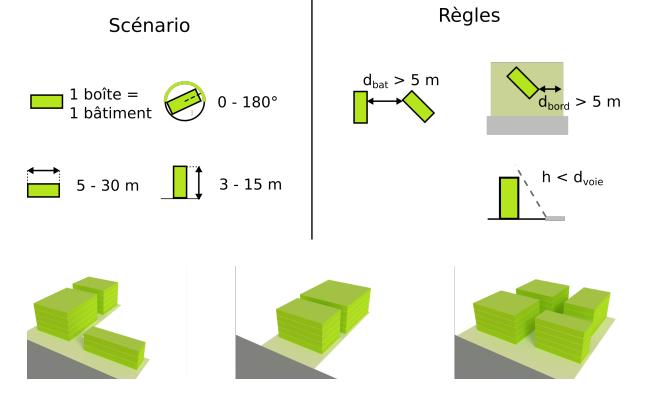
\includegraphics[width=\linewidth]{figures/simplu.png}

}


\sframe{The ParcelManager model to split parcels}{

\footnotesize

The ParcelManager model provides several algorithms for a realistic splitting of parcels with road network access \cite{colomb2022parcel}


\smallskip

\centering

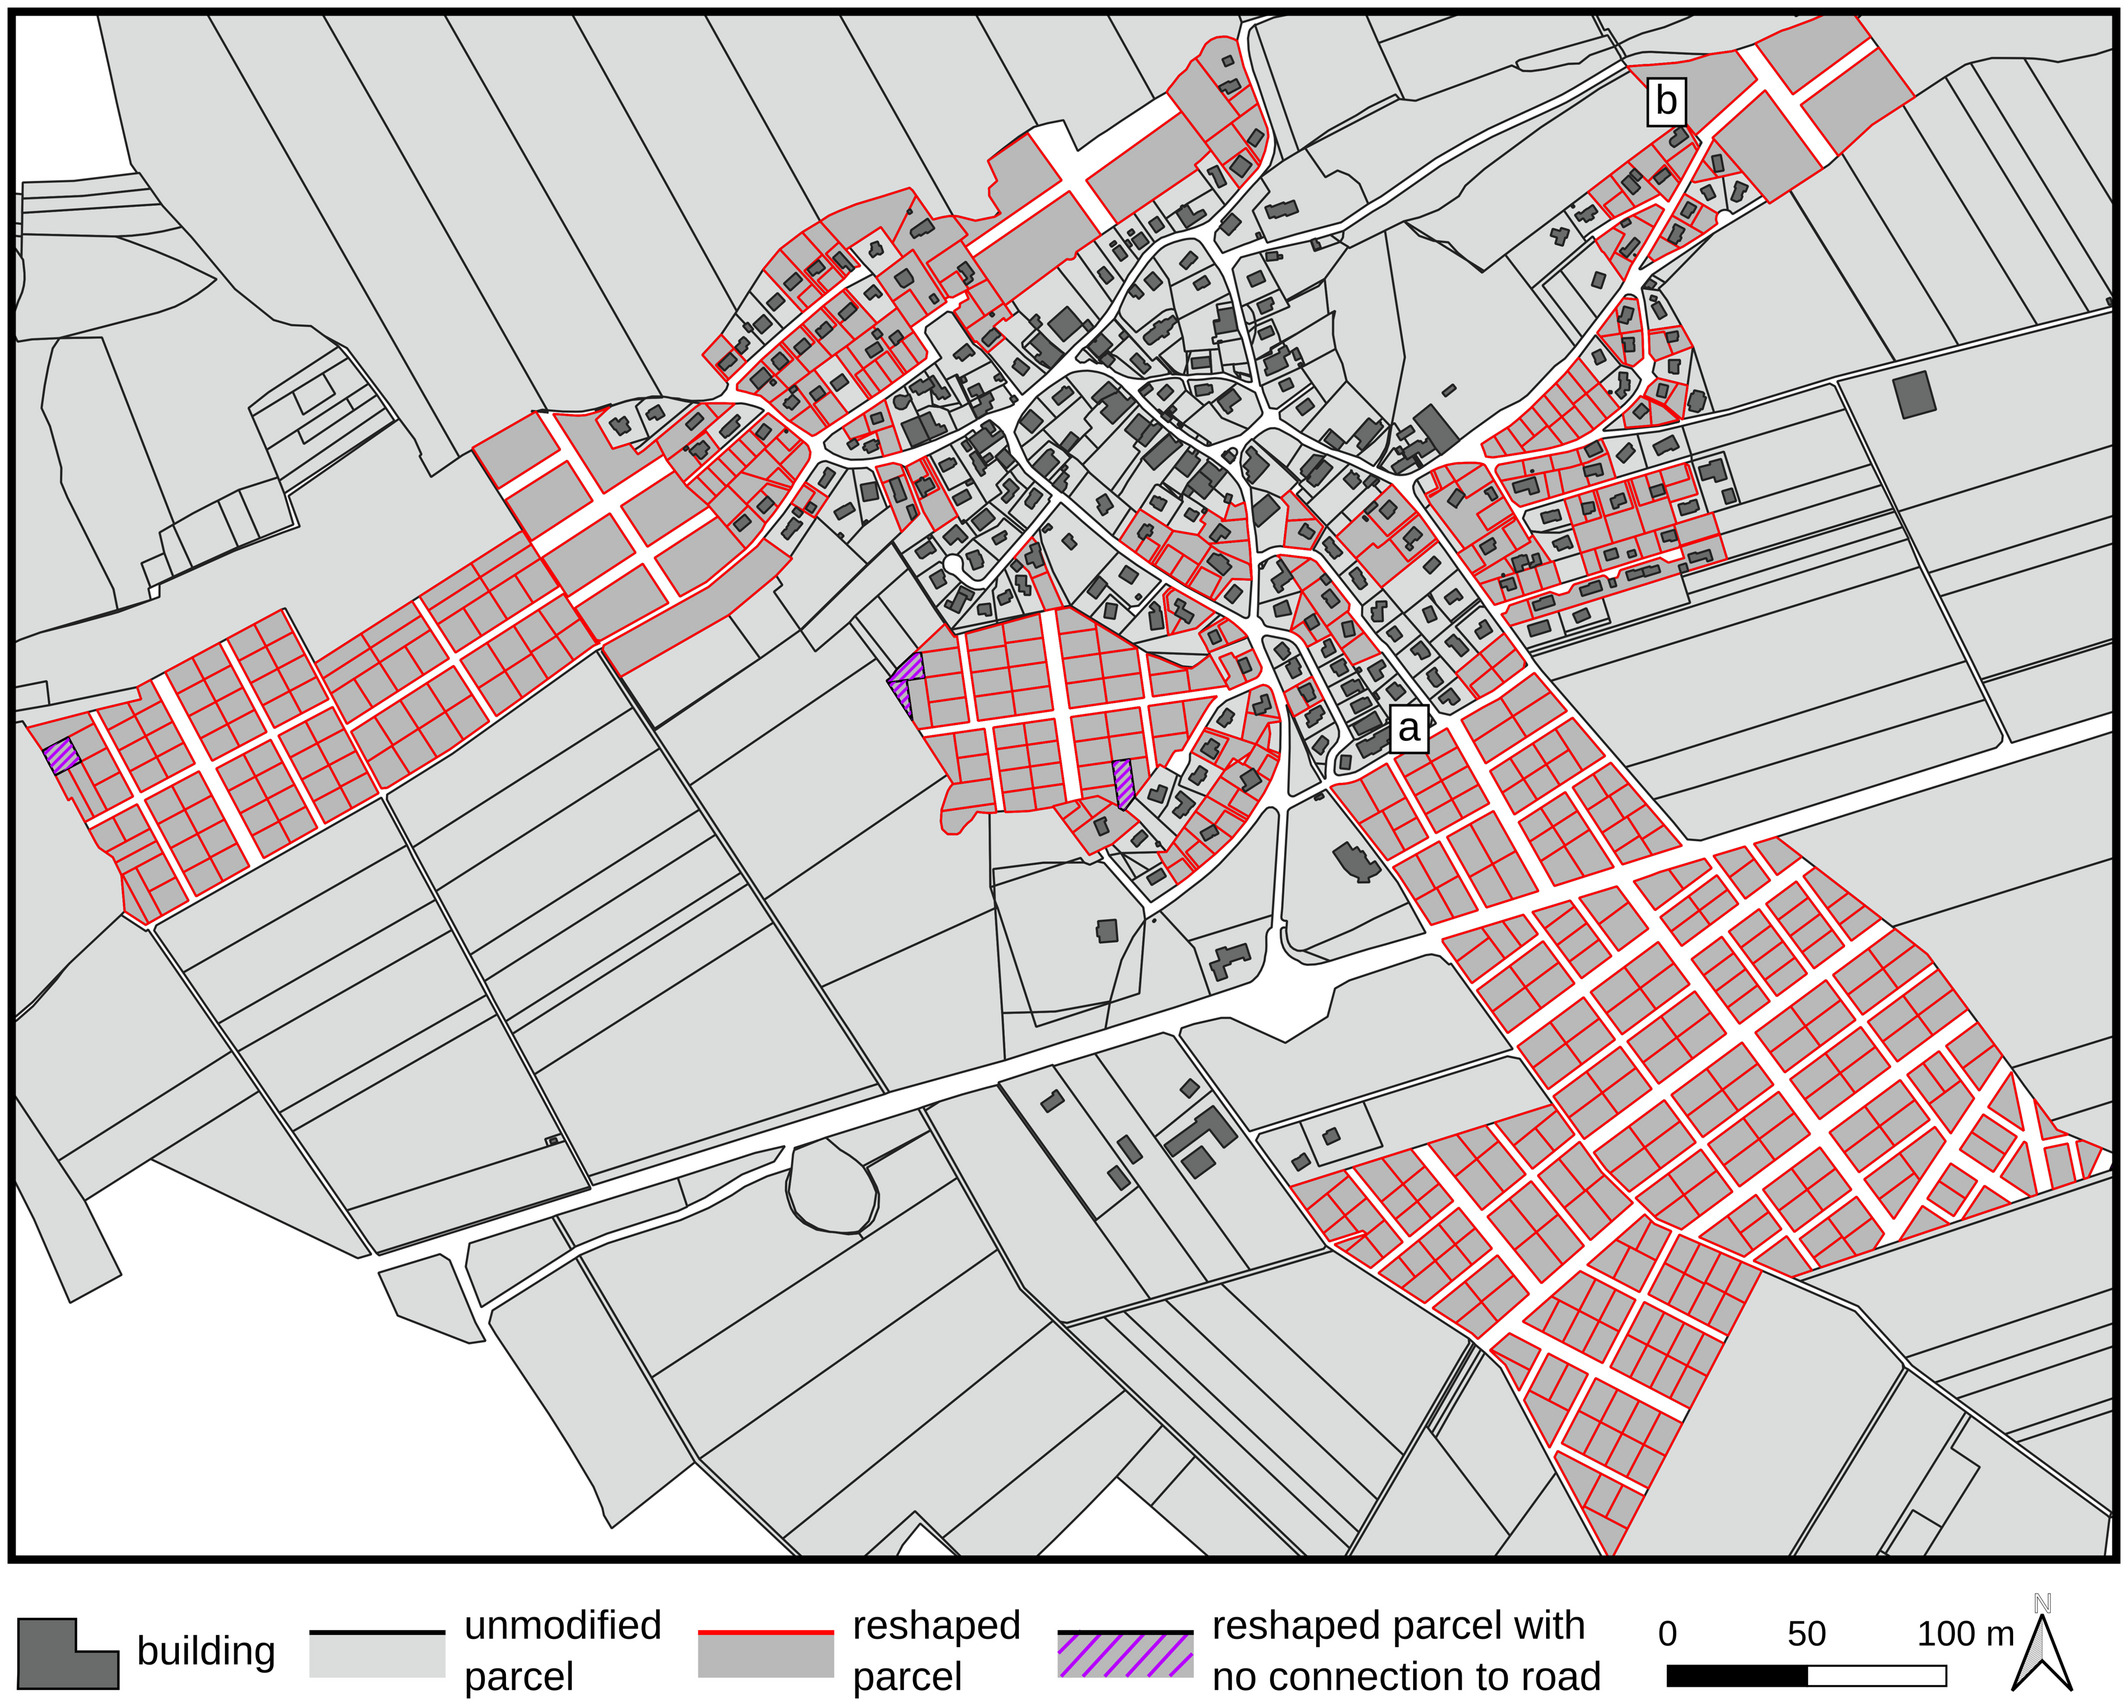
\includegraphics[width=0.8\linewidth]{figures/parcelmanager.jpg}



}


\sframe{Open issues and next steps}{

\footnotesize

\textbf{Open issues to sort out before continuing the model:}

\begin{itemize}
	\item Application of SimPLU3D to the German (explicit plan regulations) and UK (case by case regulations) contexts (already applied to the US)
	\item Which level of economic processes (price and market model, behavior of agents)?
	\item Genericity of developers and authorities across countries?
\end{itemize}

\bigskip

\textbf{Next steps:}

\begin{itemize}
	\item Discussion with qualitative researchers and insights from fieldwork surveys in the three countries
	\item Systematic review of potential processes to be included, first version to be implemented
	\item Exploration on synthetic data to explore stylised policies \cite{kang2023exploring}
	\item Application to case studies of the Subdense project
	\item Calibration on observed densification dynamics
\end{itemize}


}


%%%%%%%%%%%%%%%%%%%%%
\begin{frame}[allowframebreaks]
\frametitle{References}
\bibliographystyle{apalike}
\bibliography{biblio}
\end{frame}
%%%%%%%%%%%%%%%%%%%%%%%%%%%%





\end{document}

